
\documentclass[final]{IEEEtran}
%\documentclass{article}
%\usepackage{fullpage}
\usepackage{amsmath, amssymb}
\usepackage{graphicx}
\usepackage{subfigure}
\usepackage[noadjust]{cite}
\newtheorem{theorem}{\textbf{Theorem}}%[section]
\newtheorem{remark}{\textbf{Remark}}%[section]
\newtheorem{lemma}{Lemma}%[section]

%\title{Saving Simulations of Fault-on Dynamics in Contingency Screening}
\title{Simulation-free Estimation of Critical Clearing Time}

\author{Thanh Long Vu, \textit{Member, IEEE}, Surour Al Araifi, \textit{Student Member, IEEE}, Mohamed Elmoursi, \textit{Senior Member, IEEE}, Konstantin~Turitsyn, \textit{Member, IEEE}% <-this % stops a space
\thanks{Thanh Long Vu and Konstantin Turitsyn are with the Department of Mechanical Engineering, Massachusetts Institute of Technology, Cambridge, MA, 02139 USA, e-mail: longvu@mit.edu and turitsyn@mit.edu.
Surour Al Araifi and Mohamed Elmoursi  are with Department of
Electrical Engineering and Computer Science, Masdar Institute, Abu
Dhabi, U.A.E., email: salaraifi@masdar.ac.ae and
melmoursi@masdar.ac.ae.
%Hsiao-Dong Chiang is with School of
%Electrical and Computer Engineering, Cornell University,  Ithaca,
%NY, USA, email: chiang@ece.cornell.edu.

}}% <-this % stops a space

 \markboth{IEEE Transactions on Power Systems,~Vol.~, No.~, June ~2015}%
 {Shell \MakeLowercase{\textit{et al.}}: Saving Simulations of Fault-on Dynamics in Contingency Screening}%

\begin{document}




\maketitle
\begin{abstract}
Contingency screening for transient stability of large scale, strongly nonlinear,
interconnected  power systems is one of the
most computationally challenging parts of Dynamic Security
Assessment and requires huge resources to perform time-domain
simulations-based assessment. To reduce computational cost of time-domain
simulations, direct energy methods have been extensively developed. 
However, these methods, as well as other existing
methods, still rely on time-consuming numerical integration of
the fault-on dynamics. This task is computationally hard, since
possibly thousands of contingencies need to be scanned and
thousands of accompanied fault-on dynamics simulations need to be
performed and stored on a regular basis. In this paper, we
introduce a way to eliminate the need for fault-on dynamics
simulations in contingency screening. This technique is based on
bounding the fault-on dynamics and applying the recently
introduced Lyapunov Function Family approach for transient
stability. In turn, a lower bound of the critical
clearing time is obtained without restoring to simulations. 
A comprehensive analysis is carried out to validate this novel 
technique on a number of IEEE test cases.
\end{abstract}

%\begin{keywords}
%Power grids, synchronization, Lyapunov method, transient stability
%analysis, robust stability
%\end{keywords}


\maketitle

\section{Introduction}
%Introduction to TSA system.

%Modern power grid is undergoing a historic transformation to the
%largest ever, strongly nonlinear, interconnected system with high
%penetration of renewable generations and ubiquitous presence of active and responsive loads,
%smart meters, and power storage. The current security and stability
%assessment systems developed several decades ago need to be
%reassessed and adopted to the new, heavily stressed power system. 
%One of the most
%preeminent challenges in establishing future Dynamic
%Security Assessment Systems is how to assess the stability and security of large
%scale power systems in real time. 

Transient stability
assessment, concerned with power systems stability/instability after contingencies, is a core
element of the Dynamic
Security Assessment Systems that monitor and allow the reliable operation of power systems around the world. 
The most straightforward and dominant approach in
industry to this problem is based on the direct time-domain simulations of transient
post-fault dynamics following possible contingencies. Rapid advances in
computational hardware made it possible to perform accurate
simulations of large scale systems possibly faster than real-time
\cite{Huang:2012il,Nagel:2013kf}. However, in practice there are usually
thousands to millions of contingencies that need to be screened on
a regular basis. As such, the computational cost for time-domain
simulations-based transient stability assessment is huge. At the same time, most of these contingencies are not critical, and thus most of computational resources are spent for assessment of contingencies that do not contribute to overall system risk.


To avoid time-consuming numerical integration of post-fault
dynamics and save the computational resources, the smarter way
nowadays is to use a combination of the direct energy approaches
and time-domain simulation
\cite{Pai:1981dv,chang1995direct,Chiang:2011eo}, in which the
non-critical contingencies will be screened by the energy method
and the remaining critical contingencies are checked by
time-domain simulations. The advantage of direct energy methods is
that it allows fast screening of the contingencies while providing
mathematically rigorous certificates of stability. After decades
of research and development, the controlling unstable equilibrium
point (UEP) method \cite{Chiang:1994ir} has been widely accepted as the
most successful method among other energy function based direct
screening methods, and is being applied in industry. This method is
based on comparing the post-fault energy with the energy at the
controlling UEP to certify transient stability.

The noticeable drawback of the controlling UEP method is the
inherent difficulty of direct identification of the controlling UEP
\cite{Chiang:2013}. The controlling UEP is defined as the first
UEP whose stable manifold is hit by the fault-on trajectory at the
exit point, i.e. the point where the fault-on trajectory meets the
actual stability boundary of the post-fault Stable Equilibrium Point (SEP). 
Note that the actual stability boundary of the SEP is generally unknown, and
thus the computation of the exit point is very complicated and
usually necessitates iterative time-domain simulations. For a given 
fault-on trajectory, the controlling UEP computation requires solving a large set
of nonlinear differential algebraic equations which is done by
numerical methods. However, with respect to these methods, e.g. Newton method,
the convergence region of the controlling UEP can be very small and irregular 
compared to that of the SEP. If an initial guess for the numerical
iteration was chosen outside the convergence region of the controlling UEP,
then the computational algorithm will result in wrong controlling
UEP, leading to unreliable stability assessment. Unfortunately, it
is extremely hard to find an initial guess sufficiently close to
the controlling UEP. Until now, the unique way to directly compute
the controlling UEP reliably is to simulate and store the fault-on
trajectory. As a consequence, the UEP controlling-based method for
contingency screening still requires fault-on dynamics simulations
for each contingency.

To the best of our knowledge, there are only a few works on
contingency screening without relying on fault-on dynamics
simulations. Particularly, in \cite{roberts2015algebraic} the
closest UEP method is exploited and an algebraic formulation of
the critical clearing time is obtained based on polynomial
approximation of the swing equations. However it is assumed that the
dynamics of the rotor angles during  the  fault  is  a  constant
positive  acceleration, which is unrealistic.




The objective of this paper is to develop novel numerical approach that can potentially alleviate the computational burden of finding the controlling UEP. We aim to achieve this objective by developing a completely simulation-free technique for estimation of critical clearing time. This technique is based on the extension of the recently
introduced  Lyapunov Functions Family (LFF) approach \cite{Vu:2014, Vu:2014acc}. The principle of this approach is to
provide transient stability certificates by constructing a
family of Lyapunov functions and then finding the best suited
function in the family for given initial states. Basically, this
method certifies that the post-fault dynamics is stable if the
fault-cleared state stays within a polytope surrounding the
post-fault equilibrium point and the Lyapunov function at the
fault-cleared state is smaller than the minimum value of Lyapunov
function over the flow-out boundary of that polytope. Therefore,
to screen the contingencies for transient stability, this method
only requires the knowledge the fault-cleared state, instead of the
whole fault-on trajectory.

Exploiting this advantage of LFF method, a technique is introduced
to bound the fault-on dynamics and thereby the fault-cleared state.
This bound leads to a transient stability certificate that only
relies on checking the clearing time, i.e. if the
clearing time is under certain threshold then the fault-cleared
state is still in the region of attraction of the original SEP and
 the post-fault dynamics
is determined stable. By this new method, a fast transient
stability assessment for a large number of contingencies can be obtained without using
any simulations. Such approach can be utilized in several power system applications, such as optimal power flow and resources
allocation problems \cite{4487649, 6575172},
where the proposed transient stability certificate can help reduce the search space by eliminating
less critical contingencies in studies.


The structure of this paper is as follows. In Section
\ref{sec:LFF} the contingency screening problem addressed 
in this paper is introduced, together with the extension of the LFF 
approach for transient stability. Section \ref{sec:certificate} 
presents the main result of this paper regarding the simulation-free algebraic estimation of the critical clearing 
time, and explains how this new stability certificate can be used in practice to 
screen contingency for transient stability without time-domain simulations of
fault-on dynamics. Finally, in Section \ref{sec:simulations} results of contingency 
screening on several IEEE test systems is presented and analyzed. 
Section \ref{sec:discussion} provides the conclusion by discussing the advantages 
of different approaches and possible ways to improve the algorithms.

\section{Lyapunov Function Family Approach for Transient Stability}
\label{sec:LFF}

In this section, we describe the Lyapunov function family approach to transient stability analysis \cite{Vu:2014}, and then extend
this family to a broader set of Lyapunov functions family, that
will be instrumental to establish the lower bound of critical
clearing time in the next section. In normal conditions, power
grids operate at a stable equilibrium point. Under some fault or
contingency scenarios, the system evolves subject to the fault-on
dynamics and moves away from the pre-fault equilibrium point.
After the fault is cleared, the system experiences the post-fault
transient dynamics. In this paper, the normal type of contingencies
is considered where a three phase fault occurs in a transmission line 
causing  a tripping to the respective line. If the line is reclosed again,
typically the pre-fault dynamics and equilibrium will be the same
as the post-fault dynamics and equilibrium, respectively.



To describe the pre-fault and post-fault dynamics, we utilize the differential structure-preserving model \cite{bergen1981structure}. 
This model naturally incorporates the dynamics of rotor angle as well as response of
dynamic load power output to frequency deviation. Though it does
not model the dynamics of voltage in the system, in comparison to
the Kron-reduction models with constant impedance loads \cite{386159} the structure of power systems and the
impact of load dynamics  are preserved in this approach. When the
losses in the power grid are ignored, the model can be expressed as:
\begin{align}
\label{eq.structure-preserving}
 m_k \ddot{\delta_k} + d_k \dot{\delta_k} + \sum_{j \in
  \mathcal{N}_k} a_{kj} \sin(\delta_k-\delta_j) = &P_{m_k},  \\
  &k=1,\dots,m,  \nonumber\\
  \label{eq.structure-preserving2}
  d_k \dot{\delta_k} + \sum_{j \in
  \mathcal{N}_k} a_{kj} \sin(\delta_k-\delta_j) = &-P^0_{d_k},  \\
  & k=m+1,\dots,n, \nonumber
\end{align}
where the first $m$ equations represent the dynamics of generators
and the remaining $(n-m)$ equations represent the dynamics of
frequency-dependent loads. With $k=1,...,m,$ then $m_k$ is
the dimensionless moment of inertia of the $k^{th}$ generator,
$d_k$ is the term representing primary frequency controller action
on the governor, and $P_{m_k}$ is the effective dimensionless mechanical
power acting on the rotor. With $k=m+1,...,n,$ then $d_k>0$ is
the constant frequency coefficient of load and $P^0_{d_k}$ is the nominal load. Here, $a_{kj}=V_kV_jB_{kj},$ where
$[B_{kj}]_{\{k,j\} \in \mathcal{E}}$ is the  susceptance matrix and
 $V_k$ represents the voltage magnitude at the $k^{th}$ bus, which is assumed to be constant. The
stationary operating condition is given by
$[\delta_1^*,\dots,\delta_n^*, 0,\dots,0]^T$ where $\delta_k$ is
solution of the power flow-like equations
\begin{align}\label{eq.operatingCondition}
\sum_{j \in
  \mathcal{N}_k} a_{kj} \sin(\delta_k-\delta_j) =P_k, \forall k=1,\dots,n,
\end{align}
where $P_k=P_{m_k}, k=1,\dots,m,$ and $P_k=-P^0_{d_k},
k=m+1,\dots,n.$ We assume that there exists a stable operating
condition where $\delta_{kj}^*<\pi/2$ for all $\{k,j\}\in
\mathcal{E}.$

In the LFF approach, the nonlinear couplings and the
linear model are separated. To do that, the state vector $x =
[x_1,x_2,x_3]^T$ is introduced which is composed of the vector of generator's
angle deviations from equilibrium $x_1 = [\delta_1 -
\delta_1^*,\dots, \delta_m - \delta_m^*]^T$, their angular
velocities $x_2 = [\dot\delta_1,\dots,\dot\delta_m]^T$, and vector
of load's angle deviation from equilibrium
$x_3=[\delta_{m+1}-\delta_{m+1}^*,\dots,\delta_n-\delta_n^*]^T$.
Let $E$ be the incidence matrix of the corresponding graph, so
that $E[\delta_1\dots\delta_n]^T =
[(\delta_k-\delta_j)_{\{k,j\}\in\mathcal{E}}]^T$. Consider matrix
$C$ such that $Cx=E[\delta_1\dots\delta_n]^T.$  Consider the
nonlinear transformation $F$ in this representation is a simple
trigonometric function $
F(Cx)=[(\sin\delta_{kj}-\sin\delta^*_{kj})_{\{k,j\}\in\mathcal{E}}]^T.$

In state space representation the system can be expressed in the
following compact form:
\begin{align}
\dot{x}_1 &=x_2 \nonumber \\
\dot{x}_2 &=M_1^{-1}D_1x_2-S_1D^{-1}E^TSF(Cx)  \\
\dot{x}_3 &= -S_2D^{-1}E^TS F(Cx) \nonumber
\end{align}
where $S=\emph{\emph{diag}}(a_{kj})_{\{k,j\}\in \mathcal{E}},
S_1=[I_{m\times m}\quad O_{m\times n-m}], S_2=[O_{n-m\times m}
\quad I_{n-m\times n-m}], D_1=\emph{\emph{diag}}(d_1,\dots,d_m),
M_1=\emph{\emph{diag}}(m_1,\dots,m_n),
D=\emph{\emph{diag}}(m_1,\dots,m_m,d_{m+1},\dots,d_n).$
Equivalently, 
\begin{equation}\label{eq.Bilinear}
 \dot x = A x - B F(C x),
\end{equation}
with the matrices $A,B$ given by the following expression:
\begin{align*}
A=\left[
        \begin{array}{ccccc}
          O_{m \times m} \qquad & I_{m \times m}  \qquad & O_{m \times n-m}\\
          O_{m \times m} \qquad & -M_1^{-1}D_1 \qquad & O_{m \times n-m} \\
          O_{n-m \times m} \qquad &O_{n-m \times m} \qquad & O_{n-m \times n-m}
        \end{array}
      \right],
\end{align*}
and $$
 B= \left[
        \begin{array}{ccccc}
          O_{m \times |\mathcal{E}|}; \quad
          -S_1D^{-1}E^TS; \quad
          -S_2D^{-1}E^TS
        \end{array}
      \right].$$
Here, $|\mathcal{E}|$ is the number of edges in the graph defined
by the susceptance matrix, or equivalently the number of non-zero
non-diagonal entries in $B_{kj}$.

\begin{figure}
\label{fig.2Bus} \centering
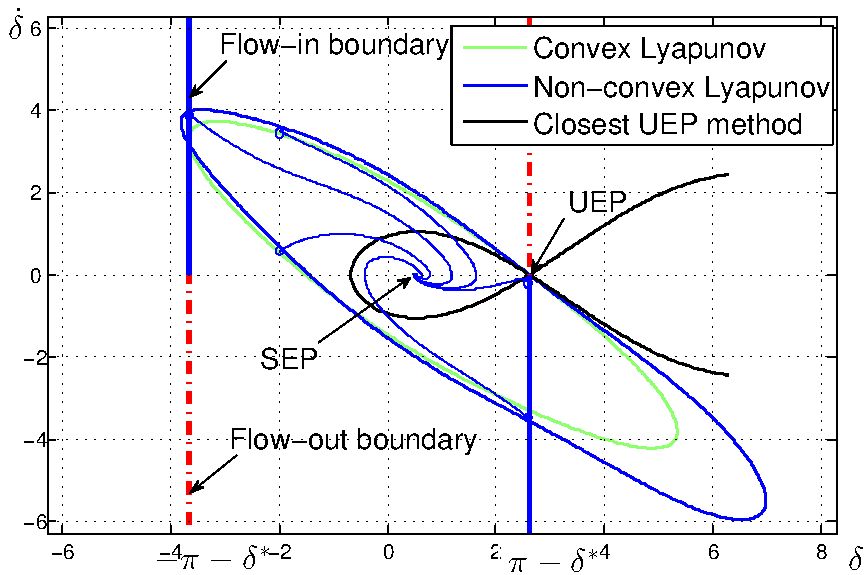
\includegraphics[width = 3.2in]{2Bus}
\caption{Estimation of the region of attraction  obtained
by the Lyapunov function family approach in comparison to that achieved by the closest UEP energy method (black solid line). There are many contingency configurations cannot be screened by the closest UEP method, but the Lyapunov function family method.}
\end{figure}

For the system defined by \eqref{eq.Bilinear}, the LFF approach
proposes to use the Lyapunov functions family  given by:
\begin{align} \label{eq.Lyapunov}
V(x) = \frac{1}{2}x^T Q x - \sum_{\{k,j\}\in \mathcal{E}}
K_{\{k,j\}} \left(\cos\delta_{kj}
+\delta_{kj}\sin\delta_{kj}^*\right)
\end{align}
in which  the diagonal matrices $K, H$ of size
$|\mathcal{E}|\times|\mathcal{E}|$ and symmetric, positive matrix
$Q$ of size $(n+m)\times (n+m)$ satisfy the LMI:
\begin{align}
\label{eq.QKH}
    \left[   \begin{array}{ccccc}
          A^TQ+QA  & R \\
          R^T  & -2H\\
        \end{array}\right] &\le 0,
%Q- \sum_{\{k,j\}\in \mathcal{E}}k_iC_i^T C_i &\ge 0.
  \end{align}
with $R = QB-C^TH-(KCA)^T$. Then, it can be proved that the
Lyapunov function is decreasing in the polytope $\mathcal{P}$
defined by inequalities $|\delta_{kj}+\delta_{kj}^*| \le \pi,
\forall \{k,j\} \in \mathcal{E}.$ In order to ensure that the
system will not escape the polytope $\mathcal{P}$ during transient
dynamics one condition will be added to restrict the set of initial
states inside $\mathcal{P}.$ Accordingly, we define the minimization
of the function $V(x)$ over the union $\partial\mathcal{P}^{out}$
of the flow-out boundary segments
$\partial\mathcal{P}_{kj}^{out}$ as follows:
\begin{align}\label{eq.Vmin1}
 V_{\min}=\mathop {\min}\limits_{x \in \partial\mathcal{P}^{out}} V(x),
\end{align}
where $\partial\mathcal{P}_{kj}^{out}$ is the flow-out boundary
segment of polytope $\mathcal{P}$ that is defined by $|\delta_{kj}
+\delta_{kj}^*| = \pi$ and $\delta_{kj}\dot{\delta}_{kj} \ge 0$.
Given the value of $V_{\min}$ the invariant set of the Lyapunov
function $V(x)$ where the convergence to equilibrium is certified
is given by
\begin{align}\label{eq.invariant}
 \mathcal{R_P} = \left\{x \in\mathcal{P}: V(x) < V_{\min}\right\}.
\end{align}


Finally, to check if the post-fault dynamics is stable, we check if the fault-cleared state
$x_0$  is inside the stability region estimate $\mathcal{R_P}$, i.e. if $x_0$ is in the polytope
$\mathcal{P}$ and $V(x_0) < V_{\min}.$ Therefore, to certify
transient stability of each contingency, the LFF approach only
need to know the fault-cleared state $x_0$ (i.e. the state of
fault-on trajectory at the clearing time), rather than the whole
fault-on trajectory.

In this paper, the proposed approach is only concerned with voltage
phase angles staying inside the polytope $\mathcal{Q}$ defined by
inequalities $|\delta_{kj}| \le \pi/2, \forall \{k,j\} \in
\mathcal{E}.$ An advantage of considering this polypote of voltage
phasor angles is that inside this polytope the Lyapunov function
$V(x)$ defined in \eqref{eq.Lyapunov} is convex. As such, the minimum 
value $V_{\min}$ can be calculated in polynomial time. In addition, a inside 
this polytope, stricter bounding can be established for the nonlinear flow vector $F$ as follows
\begin{align}
(f_{\{k,j\}}-(\delta_{kj}-\delta_{kj}^*))(f_{\{k,j\}}-\beta(\delta_{kj}-\delta_{kj}^*))
\le 0
\end{align}
where $0<\beta \le\min_{\{k,j\}\in
\mathcal{E}}\dfrac{1-\sin\delta_{kj}^*}{\pi/2-\delta_{kj}^*}$ and
$f_{\{k,j\}}=\sin\delta_{kj}-\sin\delta_{kj}^*$ is an element of
the vector $F.$ Exploiting this strict bound of the nonlinear flow
vector $F,$ the LMI \eqref{eq.QKH} can be replaced by the following
less restrictive LMI:
\begin{align}
\label{eq.NewQKH}
    &\left[   \begin{array}{ccccc}
          A^TQ+QA-2\beta C^THC   & \tilde{R} \\
          \tilde{R}^T  & -2H\\
        \end{array}\right] \le 0, \\
       & \tilde{R}=QB-(1+\beta)C^TH-(KCA)^T, \nonumber
%Q- \sum_{\{k,j\}\in \mathcal{E}}k_iC_i^T C_i &\ge 0.
  \end{align}
while all the above results for the stability certificate still
hold true. In particular, the estimate for region of attraction is
given by
\begin{align}\label{eq.RoAestimate}
 \mathcal{R_Q} = \left\{x \in\mathcal{Q}: V(x) < V_{\min}\right\}
\end{align}
with 
\begin{align}
\label{eq.Vmin2}
V_{\min}=\mathop {\min}\limits_{x \in
\partial\mathcal{Q}^{out}} V(x).
\end{align} 
The proof of this fact is given
in Appendix \ref{appen.NewQKH}. With the less restrictive LMI
\eqref{eq.NewQKH}, a broader family of Lyapunov functions can be obtained,
which will be exploited to establish the lower bound of the
critical clearing time in the next section.




\section{Contingency Screening without Time-domain Simulations}
\label{sec:certificate}

In this section, the contingency screening for
transient stability is described  by combining the LFF approach and the bounding
of the fault-on dynamics, which will completely remove any
time-domain simulations of both the post-fault dynamics and fault-on dynamics. The resulting stability certificate will only rely on checking the clearing
time.

\subsection{Bounding of The Fault-on Dynamics}

If the time-domain simulation for fault-on dynamics is used, the fault-cleared 
state $x_0$ can be determined by directly
integrating the fault-on dynamics. Then, the value of $V_0 =
V(x_0)$ computed from \eqref{eq.Lyapunov} is compared to
the value of $V_{\min}$ to certify transient stability.
%Whenever $x_0 \in
%\mathcal{P}$ and $V (x_0) < V_{\min}$ the fault-cleared state
%$x_0$ is certified to converge to the equilibrium point. If,
%however $x_0 \notin \mathcal{P}$ or $V(x_0) \ge V_{\min}$, no guarantees of convergence can be
%provided but the loss of stability or convergence to another
%equilibrium cannot be concluded as well. These configurations
%cannot be screened by a given Lyapunov function and should be
%assessed with other Lyapunov functions in the family defined by LMIs \eqref{eq.QKH} or by direct simulations of
%post-fault dynamics.

Now, assume that time-domain simulations are not used to
integrate the fault-on dynamics. Then the fault-cleared state
$x_0$ will not be known precisely. To guarantee that $x_0 \in
\mathcal{Q}$ and $V (x_0) < V_{\min},$ we will bound the fault-on dynamics. Consider the normal condition when the
pre-fault system is in the stable operating condition defined by
the SEP $x^*,$ and then a fault occurs to trip the line $\{u,v\}$.
Furthermore, assume that during the fault the parameters $P_k$
are unchanged. Then, if the fault is cleared and the line $\{u,v\}$ is reclosed,
%(Although the algorithm can easily handle cases with line tripping),
the post-fault dynamics will have the stable equilibrium point exactly at the
same as the pre-fault equilibrium point $x^*.$ The fault-on dynamics is described by
\begin{align}
\label{eq.fault-on}
\dot{x}_F=Ax_F-BF(Cx_F)+BD_{\{u,v\}}\sin\delta_{{uv}_F}
\end{align}
where the fault-on trajectory is denoted as $x_F(t)$ to
differentiate it from the post-fault trajectory $x(t)$ in
\eqref{eq.Bilinear}, and $D_{\{u,v\}}$ is the unit vector to
extract the nonlinear function
$(\sin\delta_{uv}-\sin\delta^*_{uv})$ from the nonlinear vector
$F$. In Appendix \ref{appendix.BoundingCondition}, the
following center result regarding the bounding of the fault-on dynamics is proven,
which will be instrumental to the introduction of stability certificate
in the next section. If there exist matrices $Q,K,H, H\ge 0$ and a
positive number $\gamma$ such that
\begin{align}
\label{eq.BoundingCondition}
    \left[   \begin{array}{ccccc}
          \tilde{A}+ \gamma (QBD_{\{u,v\}})(QBD_{\{u,v\}})^T  & \tilde{R} \\
          \tilde{R}^T  & -2H\\
        \end{array}\right] &\le 0,
%Q- \sum_{\{k,j\}\in \mathcal{E}}k_iC_i^T C_i &\ge 0,
  \end{align}
where $\tilde{A}=A^TQ+QA - 2\beta C^THC,\tilde{R} =
QB-(1+\beta)C^TH-(KCA)^T$, then along the fault-on dynamics
\eqref{eq.fault-on} we have $\dot{V}(x_F(t)) \le
\dfrac{1}{2\gamma}$ whenever $x_F(t)$ being in the polytope
$\mathcal{Q}.$




Note that the Lyapunov function's derivative $\dot{V}(x)$ along
the pre-fault dynamics \eqref{eq.Bilinear} is non-positive in the
polytope $\mathcal{Q}.$ Basically, the above result provides a
certificate to make sure that the fault-on dynamics does not
deviate too much from the pre-fault dynamics. As such, if the
clearing time is under some threshold, then the fault-cleared
state (i.e. the state of fault-on system at the clearing time) is
not very far from the considered working condition. The above
result as such is essential to establish a lower bound of the
critical clearing time in the next section.


To solve the inequality \eqref{eq.BoundingCondition}, we note that
for a fixed value of $\gamma,$ the inequality
\eqref{eq.BoundingCondition} can be transformed to the following
LMI of the matrices $Q,K,H$ via Schur complement:
\begin{align}
\label{eq.BoundingConditionLMI}
    \left[   \begin{array}{ccccc}
          A^TQ+QA-2\beta C^THC   & (\sqrt{\gamma}(QBD_{\{u,v\}}) \;\; \tilde{R}) \\
          (\sqrt{\gamma}(QBD_{\{u,v\}}) \;\;\tilde{R})^T  & -L\\
        \end{array}\right] &\le 0,
  \end{align}
  where $L=\left[   \begin{array}{ccccc}
          I   & O \\
          O  & 2H\\
        \end{array}\right].$
The matrices $Q,K,H$ can be found quickly from the LMI
\eqref{eq.BoundingConditionLMI} by convex optimization. Therefore,
a heuristic algorithm can be used to find solution of
\eqref{eq.BoundingCondition}, in which $\gamma$ is varied and 
the LMI \eqref{eq.BoundingConditionLMI} is solved to obtain the
matrices $Q,K,H$ accordingly.

\subsection{Estimation of The Critical Clearing Time}
\label{sec.EstimationCCT}

Let the clearing time be $\tau_{clearing}.$ In Appendix
\ref{appendix.ClearingTimeCertificate}, the following
stability certificate which only relies on checking the clearing
time is proven. If the inequality \eqref{eq.BoundingCondition} holds and the
clearing time $\tau_{clearing}$ satisfies $\tau_{clearing}<
2\gamma (V_{\min}-V(x^*)),$  then, the fault-cleared state
$x_F(\tau_{clearing})$ is still inside the region of attraction of
the post-fault SEP $x^*$ and the post-fault dynamics following the
considered contingency leads to the stable operating condition
$x^*$. 

Therefore, this stability certificate provides us with a lower bound of the critical clearing
time as $2\gamma (V_{\min}-V(x^*))$ obtained by solving the inequality
\eqref{eq.BoundingCondition} and calculating the minimum value
$V_{\min}.$ This estimation of the critical clearing time is
totally simulation-free,  distinguishing it from other methods
in the literature to find the critical clearing time.

\begin{figure}[t!]
\centering
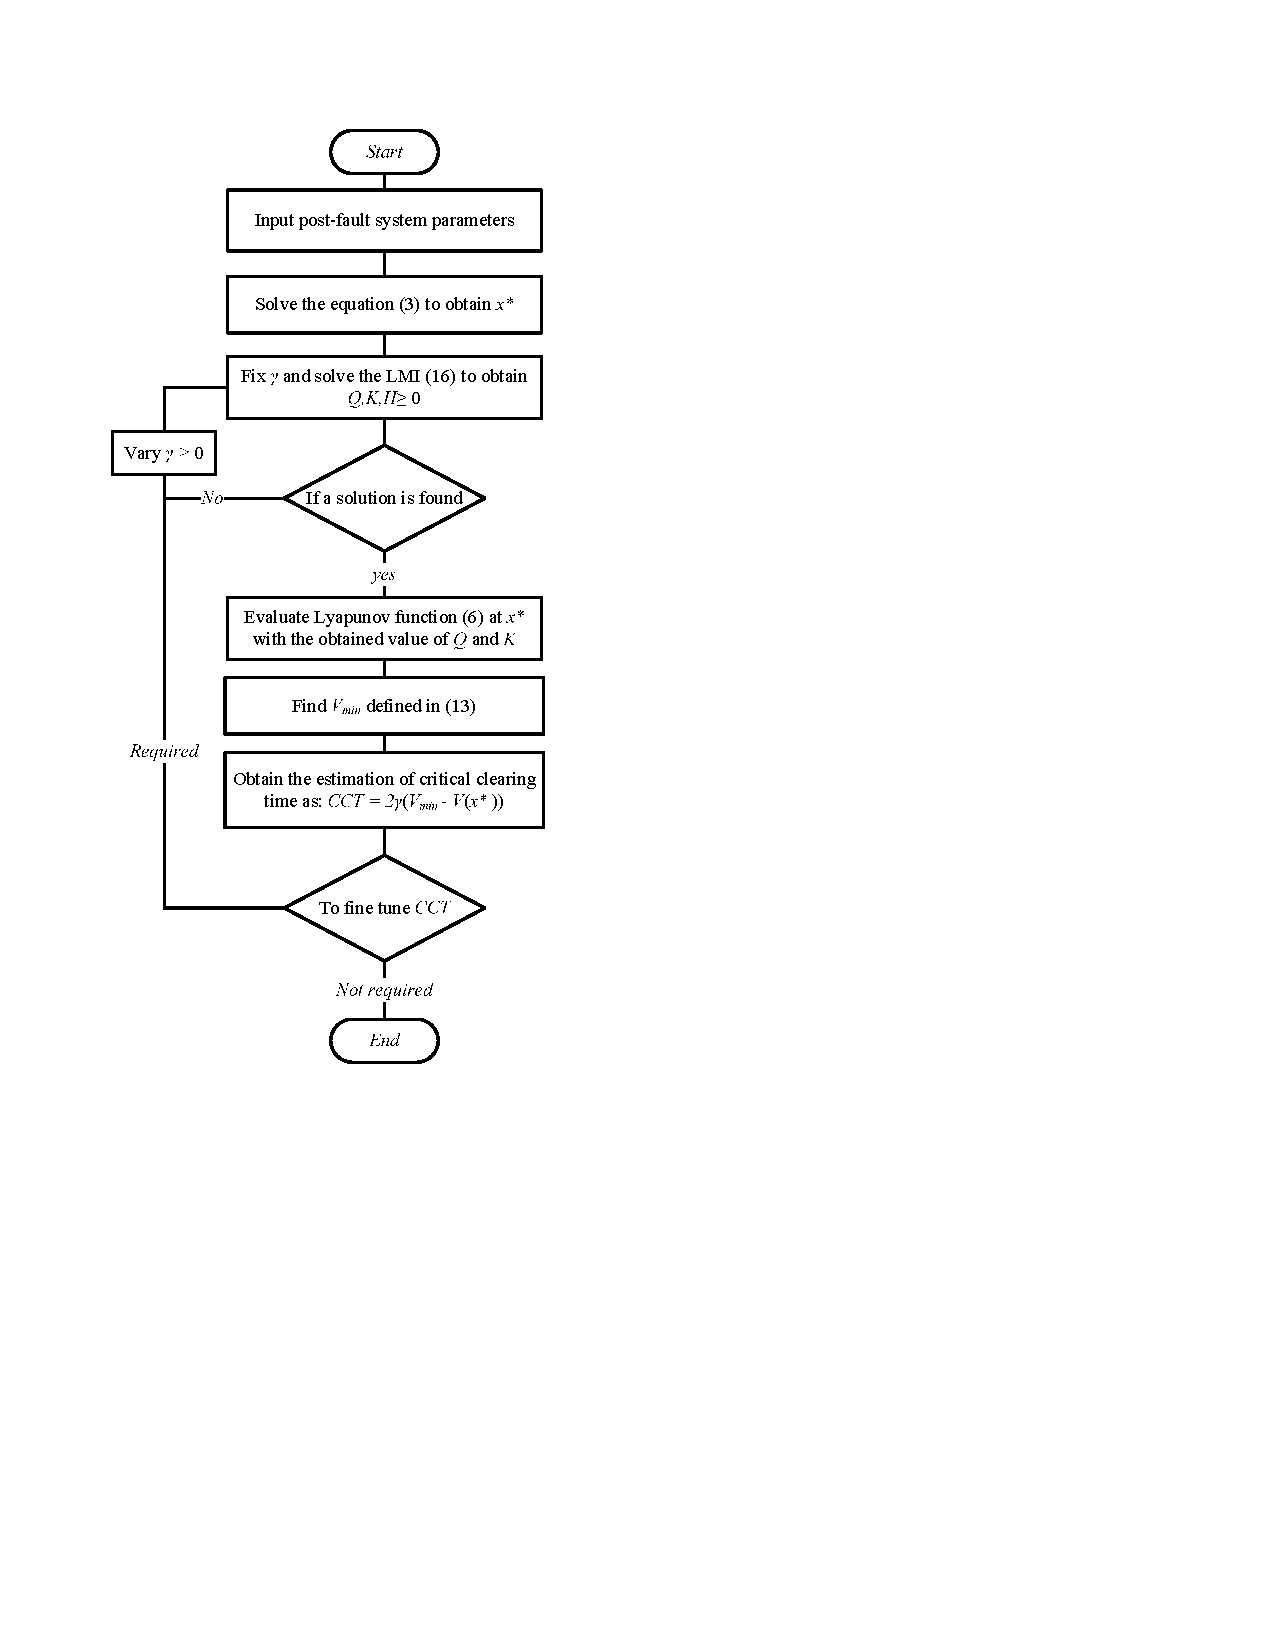
\includegraphics[width = 2.8in]{Flowchart}
\caption{Algorithm to screen contingencies for transient stability without simulations}\label{flowchart}
\end{figure}


We note that the pre-fault dynamics and post-fault dynamics are
not necessary the same. The proposed technique is easy to extend
to the case when these dynamics as well as the pre-fault SEP and
post-fault SEP are different. Particularly, the lower bound of the
critical clearing time $2\gamma (V_{\min}-V(x^*))$ will be replaced by the
new bound $2\gamma (V_{\min}-V(\emph{\emph{SEP}}_{pre-fault})).$ The proof is
straightforward and omitted here.

It is also possible to extend this stability certificate to the
case when several contingencies co-exist. This case is of
practical interest. Indeed, the large-area blackout in practice is
usually  a result of multiple contingencies happening at short time interval.
Though large-area blackout is rare, its effect is severe,
both economically and humanly. Therefore, it is critical  to check
if the power grids stand when several contingencies are happening,
or leading to large-area blackout. The technique presented in this
paper provides a framework to certify the safety of power grids.







\subsection{Contingency Screening without Simulations}


The stability certificate in the previous section provides us with
a way to directly screen contingencies for transient stability assessment
without any time-domain simulations, as described by the algorithm in Fig. \ref{flowchart}. Basically, for the
contingency manifested by the tripping of line $\{u,v\},$ one can
check if the inequality \eqref{eq.BoundingCondition} is solvable.
In case it is solvable to find the matrices $Q,K,H,$
and the positive number $\gamma,$ then the Lyapunov
function $V(x)$ can be derived as in \eqref{eq.Lyapunov}, and the minimum
value $V_{\min}$ defined in \eqref{eq.Vmin2} can be calculated. Finally, if the
clearing time satisfies that $\tau_{clearing}<2\gamma (V_{\min}-V(x^*)),$ 
then we conclude that the
post-fault dynamics following the considered contingency leads to
a stable operating condition. If this inequality is not true, or
if there is no solution for the inequality
\eqref{eq.BoundingCondition}, then nothing can be concluded 
about the stability or instability of the post-fault dynamics. The
contingency in this case should be screened by other method or by
direct time-domain simulations.


Note that the large family of possible Lyapunov functions,
given by the matrices $Q,K,H$ satisfying the inequality
\eqref{eq.BoundingCondition}, gives us the flexibility in
contingency screening. Accordingly, an efficient adaptation algorithm for finding the
Lyapunov functions can be developed to a given contingency in the same spirit with
the adaptation algorithm proposed in \cite{Vu:2014}. Then, with the
contingency scenario presented as a fault on the line
$\{u,v\}$, the most suitable Lyapunov functions can be found in the
family defined by the inequality \eqref{eq.BoundingCondition}, that
will give us the estimation  $2\gamma (V_{\min}-V(x^*))$ of the 
critical clearing time as large as possible, as showed in Table
\ref{tab.CCT} for the simple case of two buses system.

\subsection{Robust Contingency Screening}

In contingency screening, it is greatly advantageous if we have a certificate to screen any possible contingency associated
with the tripping of any line in $\mathcal{E}$. Let $D$ be a
matrix larger than or equal to $D_{\{u,v\}}D_{\{u,v\}}^T$ for all
the lines $\{u,v\}\in \mathcal{E}.$ We have the following result
for the robust screening of contingencies.
If the inequality
\eqref{eq.BoundingCondition} holds with $D_{\{u,v\}}D_{\{u,v\}}^T$
replaced by $D$, and the clearing time $\tau_{clearing}$ satisfies
$\tau_{clearing}< 2\gamma (V_{\min}-V(x^*)),$  then, for any contingency associated with the
tripping of any line $\{u,v\}\in \mathcal{E},$ the fault-cleared state
$x_F(\tau_{clearing})$ is still inside the region of attraction of
the post-fault SEP $x^*$, and the post-fault dynamics following
the considered contingency leads to the stable operating condition
$x^*$. This result is a straightforward corollary of the stability
certificate in Section \ref{sec.EstimationCCT}, and thus its proof
is omitted here.




\section{Numerical Illustrations}
\label{sec:simulations}

\subsection{Classical 2 bus system}
\begin{figure}[t!]
\centering
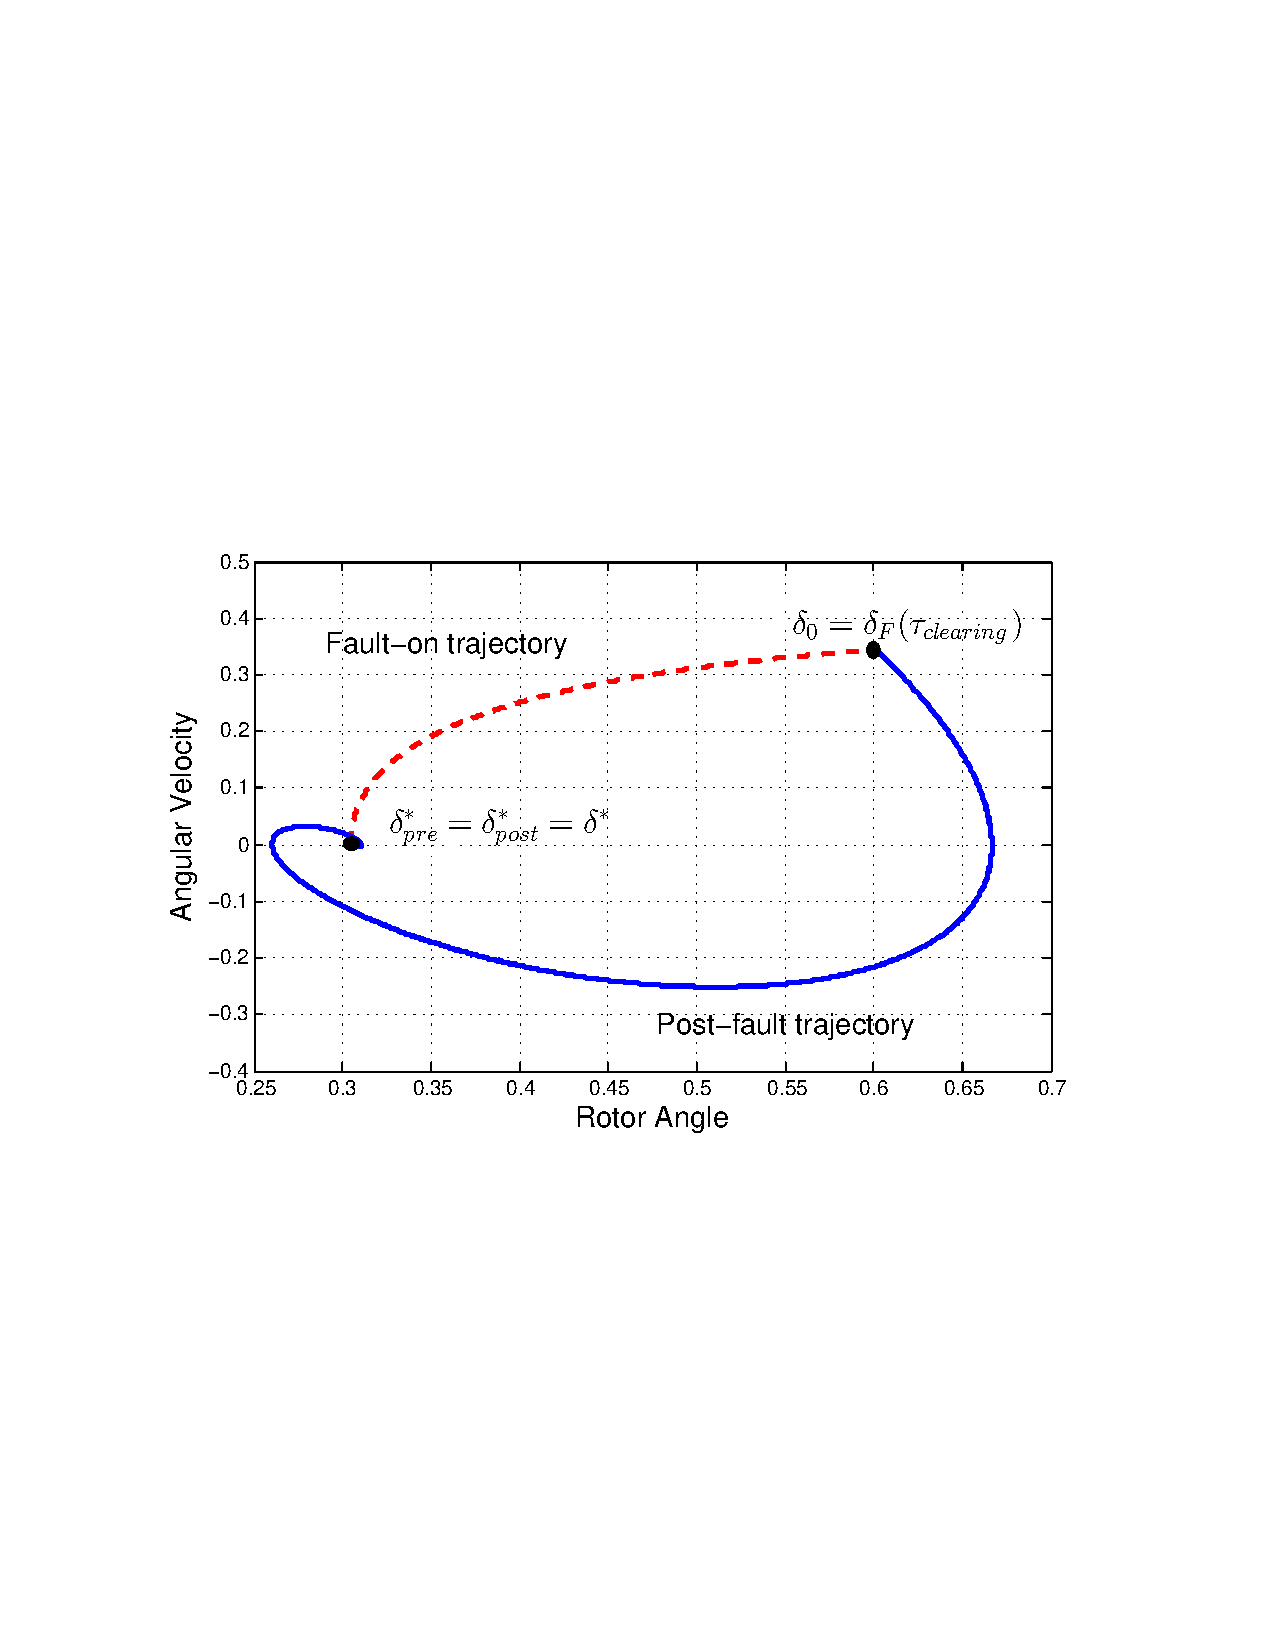
\includegraphics[width = 3.2in]{Faulton_1machine}
\caption{System trajectory according to the fault-on dynamics and
post-fault dynamics with the clearing time $CT=2\gamma
(V_{\min}-V(x^*))=1.3189 s$} \label{fig.Trajectory}
\end{figure}

\begin{figure}[t!]
\centering
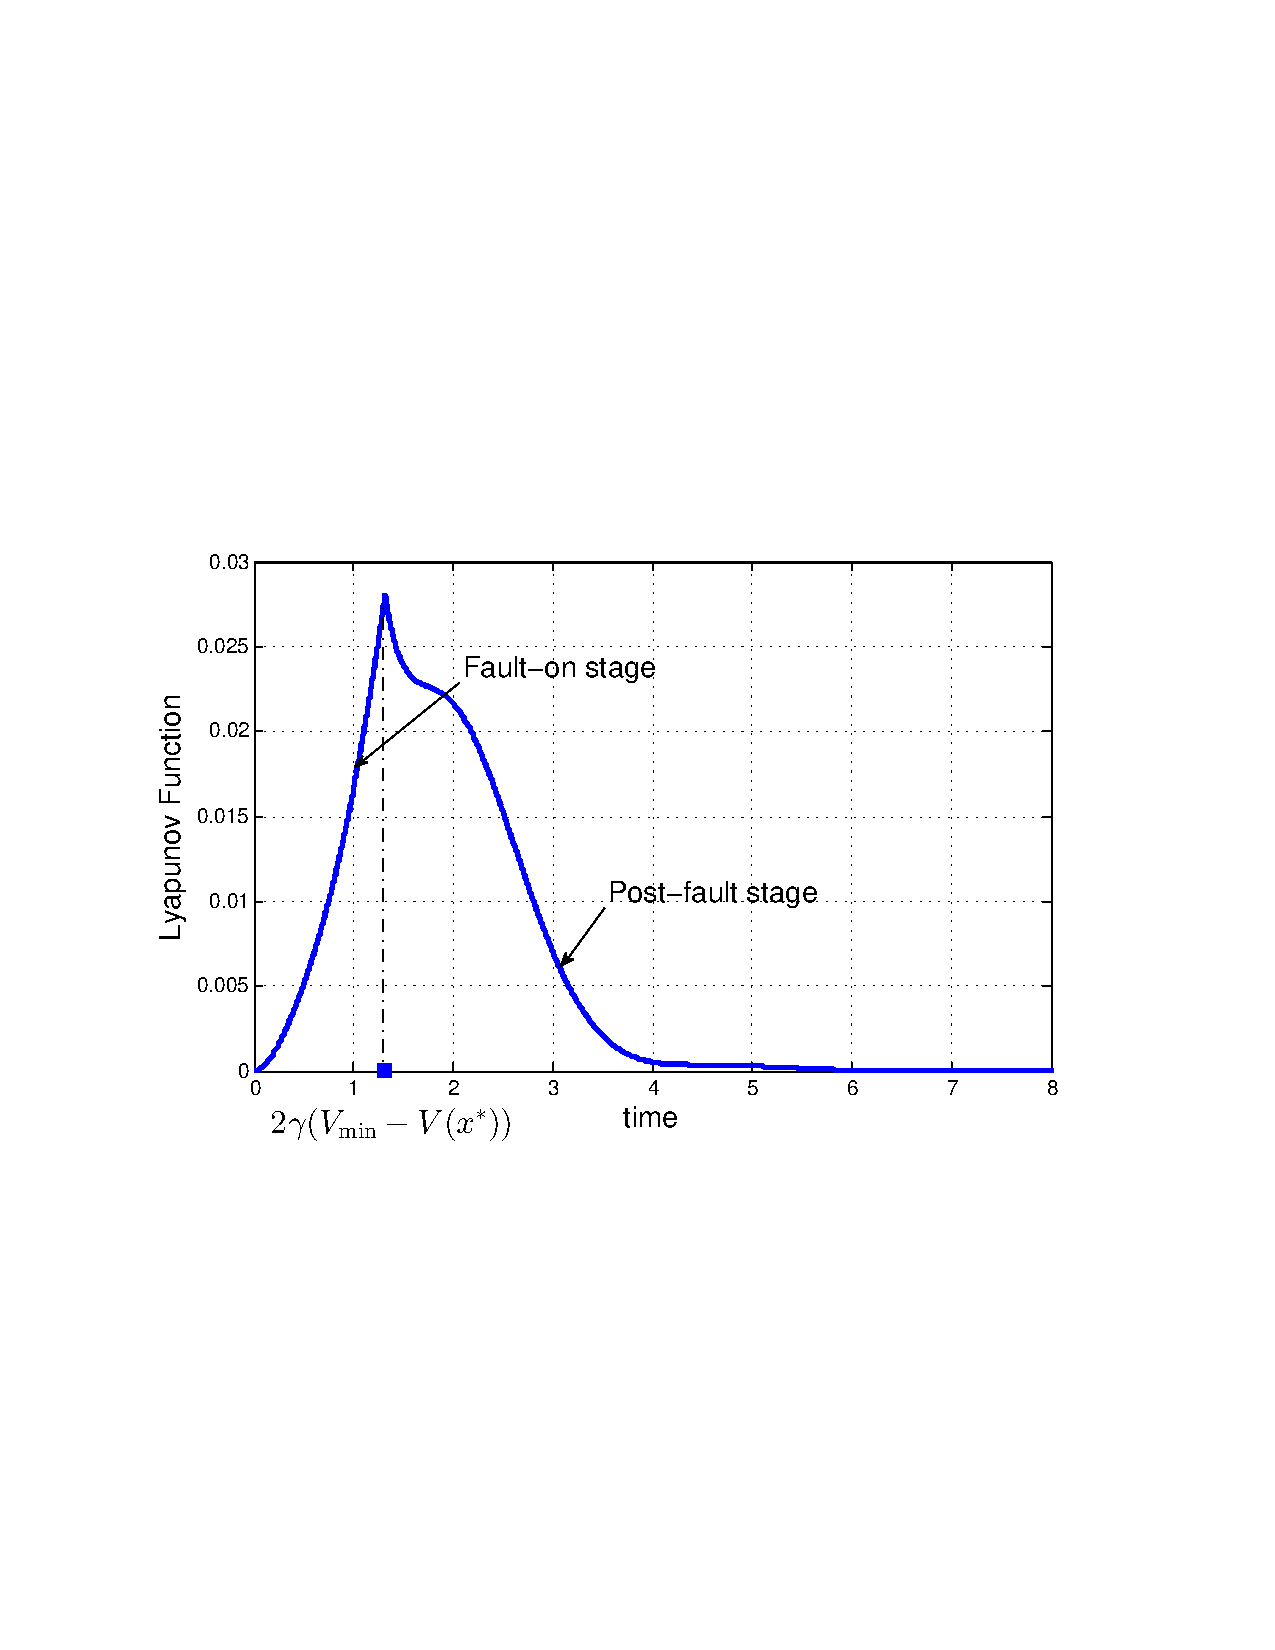
\includegraphics[width = 3.2in]{FaultonLyapunov_1machine}
\caption{Dynamics of the Lyapunov function during the fault-on
stage and post-fault stage with the clearing time $CT=2\gamma
(V_{\min}-V(x^*))=1.3189 s$} \label{fig.Lyapunov}
\end{figure}

For illustrating the presented concepts, this section presents the
simulation results on the most simple 2-bus power system,
described by the single 2-nd order differential equation
\begin{align}
  m \ddot{\delta} +d \dot{\delta} + a \sin\delta - p=0.
\end{align}
For numerical simulations, we choose $m=0.1$ p.u., $d=0.15$ p.u.,
$a= 0.2$ p.u., and $p=0.06$ p.u. Then the stable equilibrium point
is given by $[\delta^* \;\;0]^T=[0.3047 \;\; 0]^T.$ Choose
$\beta=0.3.$ By varying $\gamma$ and solving the LMI
\eqref{eq.BoundingConditionLMI}, we obtain the corresponding lower
bounds for the critical clearing time as in the table
\ref{tab.CCT}.

\begin{table}[ht!]
\centering
\begin{tabular}{|c|c|}
  \hline
  % after \\: \hline or \cline{col1-col2} \cline{col3-col4} ...
  $\gamma$ & $2\gamma (V_{\min}-V(x^*)) (s)$ \\
  \hline
  0.1  & 0.8061 \\
  1 & 0.9652 \\
  2 & 1.1229 \\
  3 & 1.3189 \\
  4 & 1.1960 \\
  5 & 1.1580\\
  10 & 0.9517\\
  \hline
\end{tabular}
\caption{Lower bound of the critical clearing time vs.
$\gamma$}\label{tab.CCT}
\end{table}

Therefore, in these values of $\gamma,$ with $\gamma=3$  we obtain
the largest lower bound for the critical clearing time as
$1.3189.$ The corresponding matrices $Q,K,H$ are
\begin{align}
Q=\left[   \begin{array}{ccccc}
          0.0037   & 0.0108 \\
          0.0108  & 0.1939\\
        \end{array}\right]; K= 0.3778;H=0.0285,
\end{align}
while the corresponding minimum value $V_{\min}$ is $0.2089.$ In
Fig. \ref{fig.Trajectory} we show the dynamics of the system
trajectory in the fault-on and post-fault-stage in which the
clearing time is taken as $\tau_{clearing}=1.3189 s.$ It can be seen
that when the line is tripped the system evolves according to the
fault-on dynamics and the system trajectory deviates from the
pre-fault equilibrium point to the fault-cleared state
$\delta_F(\tau_{clearing}).$ When the fault is cleared and the
line is re-closed, the system trajectory recovers from the
fault-cleared state to the post-fault equilibrium point which is
the same with the pre-fault equilibrium. Figures
\ref{fig.Lyapunov} shows the increase of the Lyapunov function
during the fault-on stage and the convergence of Lyapunov function
during the post-fault stage. These figures confirm the estimation
of the critical clearing time as obtained by the proposed method
in this paper.



\subsection{Three generator system}

Consider the system of three generators with the time-invariant
terminal voltages and mechanical torques given in Tab.
\ref{tab.data3machine}.

\begin{table}[ht!]
\centering
\begin{tabular}{|c|c|c|}
  \hline
  % after \\: \hline or \cline{col1-col2} \cline{col3-col4} ...
  Node & V (p.u.) & $P_k$ (p.u.) \\
  \hline
  1 & 1.0566 & -0.2464 \\
  2 & 1.0502 & 0.2086 \\
  3 & 1.0170 & 0.0378 \\
  \hline
\end{tabular}
\caption{Voltage and mechanical input} \label{tab.data3machine}
\end{table}

The susceptances of the transmission lines are $B_{12}=0.739$ p.u.,
$B_{13}=1.0958$ p.u., and $B_{23}=1.245$ p.u. The equilibrium
point is calculated as: $\delta^*=[-0.2057\;
   -0.2048 \;
   -0.2051 \;0\;0\;0]^T.$ Choose $\beta=0.3.$ For simplicity we just take $m_k=2,d_k=1, k=1,2,3.$ Assume that the fault trips the line between
   generators $1$ and $2$ and when the fault is cleared the line is re-closed. Also, during that time the mechanical inputs are assumed to be unchanged. Taking $\gamma=3$ and using CVX software we can solve the LMI
   \eqref{eq.BoundingConditionLMI} we obtain
   \begin{align}
   Q=\left[%
\begin{array}{cccccc}
    3.8376  &  3.8012 &   3.5779  &  7.5549  &  7.4619  &  7.4166 \\
    3.8012  &  3.8457  &  3.5698  &  7.4776  &  7.5530  &  7.4029 \\
    3.5779  &  3.5698  &  4.0690  &  7.4010  &  7.4185  &  7.6140 \\
    7.5549  &  7.4776  &  7.4010  & 38.9402  & 38.2449  & 38.0704 \\
    7.4619  &  7.5530  &  7.4185  & 38.2449  & 38.9534  & 38.0571 \\
    7.4166  &  7.4029  &  7.6140  & 38.0704  & 38.0571  & 39.1280 \\
    \end{array}%
\right]
   \end{align}
   and $K= \emph{\emph{diag}}(0.2554,
   \;       0.3638,
   \;       0.4386), H=  \emph{\emph{diag}}(0.0943,0.2533,0.2960).$ The corresponding power bound of the critical clearing time is $2\gamma (V_{\min}-V(x^*))= 0.2376 s.$

\subsection{Kundur 9 bus 3 generator system}
\begin{figure}[t!]
\centering
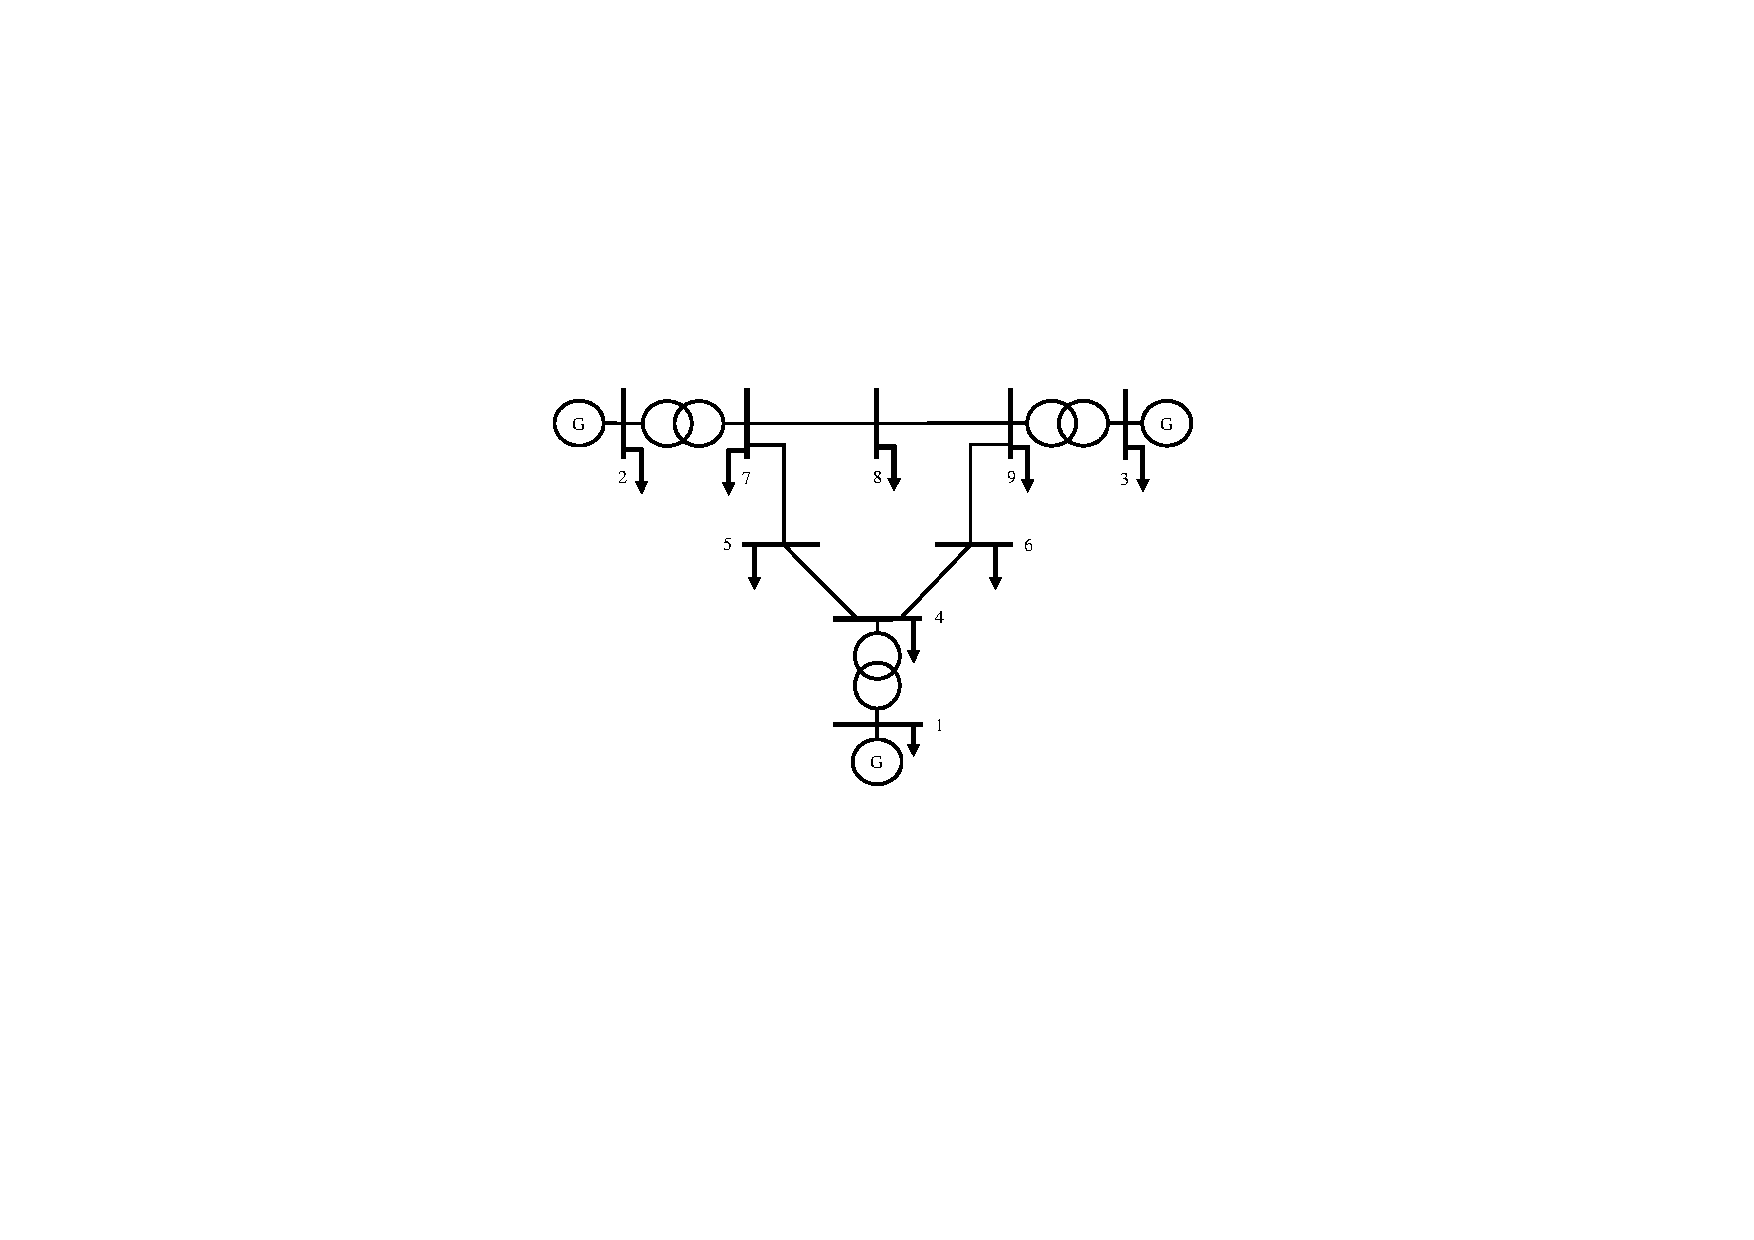
\includegraphics[width = 3.2in]{3generator9bus}
\caption{3 generator 9 bus system with frequency-dependent dynamic loads} \label{fig.3generator9bus}
\end{figure}

Consider the Kundur 9 bus 3 machine system depicted in Fig. \ref{fig.3generator9bus}  with the susceptances of the transmission lines as follows:
$B_{14}=17.3611 p.u.,B_{27}=16.0000 p.u.,B_{39}= 17.0648 p.u., B_{45}=11.7647 p.u., B_{57}= 6.2112p.u., B_{64}=10.8696p.u.,
B_{78}= 13.8889p.u.,B_{89}=9.9206p.u., B_{96}=5.8824p.u.$ The bus voltages $V_k$, mechanical inputs $P_{m_k}$, and steady state load $-P_{d_k}^0$ are given in the
Tab. \ref{tab.data9bus}. The stable operating condition is obtained by solving equations \eqref{eq.operatingCondition}
as $x^*=[0.0381\;
    0.3208\;
    0.1924\;
   -0.0349\;
   -0.0421\;
   -0.0409\;
    0.0519\;
    0.0178\;
    0.0155\; 0\; 0\; 0\; 0\; 0\; 0\; 0\; 0\; 0].$ The parameters for generators are $m_1=0.1254, m_2=0.034, m_3=0.016, d_1=0.0627, d_2=0.017, d_3=0.008.$ For simplicity, we take $d_k=0.05, k=4\dots,9.$ Assume that the fault trips the line between buses $6$ and $4$ and when the fault is cleared this line is re-closed. With $\beta=0.3, \gamma=10^{-5}, $ using the CVX software, we can solve the LMI
   \eqref{eq.BoundingConditionLMI}. Accordingly, we can calculate the minimum value of the Lyapunov function and obtain the lower bound for the critical clearing time as $2\gamma (V_{\min}-V(x^*))=0.1049 s.$
\begin{table}[ht!]
\centering
\begin{tabular}{|c|c|c|}
  \hline
  % after \\: \hline or \cline{col1-col2} \cline{col3-col4} ...
  Node & V (p.u.) & $P_k$ (p.u.) \\
  \hline
  1 & 1.0284 & 0.6700 \\
  2 & 1.0085 & 1.6300 \\
  3 & 0.9522 &  0.8500 \\
  4 & 1.0627 & -0.5000 \\
  5 & 1.0707 & -0.7500 \\
  6 & 1.0749 & -0.4500 \\
  7 & 1.0490 & -0.4500 \\
  8 & 1.0579 &  -0.5000 \\
  9 & 1.0521 &  -0.5000 \\
  \hline
\end{tabular}
\caption{Bus voltages, mechanical inputs and static loads}\label{tab.data9bus}
\end{table}


\section{Conclusions and Path Forward}
\label{sec:discussion}

In this paper, we introduced techniques to screen contingencies
for transient stability without relying on any time-domain simulations. This is based on extending the recently introduced LFF transient
stability certificate in the combination with bounding of the fault-on dynamics.
Basically, the LFF approach can certify the post-fault dynamics's
stability when the fault-cleared state is in some polytope
surrounding the post-fault stable operating point and the Lyapunov
function at the fault-cleared state is under some threshold. We
observed that the LFF certificate only needs to know the
fault-cleared state, instead of the fault-on trajectory.
Therefore, with the introduced bounding technique we can bound the
Lyapunov function at the fault-cleared state, by which we certify
stability for a given contingency scenario without involving any
simulations for the fault-on trajectory and post-fault trajectory.
In turns, we obtain an algebraic formulation for the lower bound of the critical
clearing time, and the stability assessment now only involves checking
if the clearing time is smaller than that lower bound to assure
the stability of the post-fault dynamics.  Remarkably, the proposed stability certificate only
relies on solving LMI and convex optimization problems, and it is therefore
scalable to stability assessment of large scale power systems, especially when combined with recent advances in semi-definite programming exploiting
the relatively low tree-width of the grids' graph \cite{Javadmadani2014sdp}.
%Our
%numerical simulations showed that this new stability certificate
%region is well applied and saves much more computational resources, comepared to the existing methods
%such as controlling UEP method.



Toward the practical applications of the proposed simulation-free
approach to contingency screening, further extensions should be
made in the future where more complicated models of power systems
are considered,
  e.g. the dynamics of generators' voltage or effects of buses' reactive power is incorporated in the model.
Since the LFF method is applicable to lossy power grid
\cite{Vu:2014acc}, it is straightforward to extend the proposed method in this paper to
incorporating reactive power, which will introduce the cosine term
in the model \eqref{eq.Bilinear}. This can be done by extending
the state vector $x$ and combining the technique in this paper
with the LFF transient stability techniques 
for lossy power grids (without reactive power considered) \cite{Vu:2014acc}. Also,
we can see that, in order to make sure the Lyapunov function is
decreasing in the polytope $\mathcal{Q},$ it is not necessary to
restrict the nonlinear terms $F(Cx)$ to be univariate. As such, we
can extend the proposed method to power systems with generators'
voltage dynamics in which the voltage variable is incorporated in
a multivariable nonlinear function $F.$

Furthermore, the proposed simulation-free contingency screening
method could be developed to robustly assess the stability of
power systems for a set of faults co-happening. This can be applied when there are significant changes in the power gird topology such as in
load shedding \cite{7077021,siddiqui2015preventive} and controlled islanding schemes
\cite{januszquiros2014constrained,6774471}. For this end, a
more restrictive bounding of the fault-on dynamics should be
employed to alleviate the conservativeness of the proposed method,
which is expected when multiple faults are considered.

%We envision to develop a new security assessment toolbox for
%practical power grids based on the LFF approach. This tool can
%certify transient stability for a broad set of contingency
%scenarios when the dynamics of power systems in described by a
%number of models, from simple classical reduction model to complex
%structure-preserving model with dynamic voltage and reactive power
%incorporated. Also, this security assessment toolbox can certify
%stability for rather complicated situations when the system
%parameters are changing or unknown via the robust stability
%certificate developed in \cite{Vu:2014acc}. We will build a
%library of models and contingency scenarios the stability of which
%can be certified by this security assessment toolbox. This will
%help us quickly assess the transient stability of dynamical power
%systems by offline algorithms.



\section{Appendix}

\subsection{Proof of the Transient Stability Certificate}
\label{appen.NewQKH}

From  the inequality \eqref{eq.NewQKH}, there exist matrices
$X_{|\mathcal{E}| \times (n+m)}, Y_{|\mathcal{E}|
\times|\mathcal{E}|}$
  such that
\begin{align}
  A^TQ+QA -2\beta C^THC = & -X^TX, \nonumber \\
  QB-(1+\beta)C^TH-(KCA)^T = &-X^TY, \nonumber \\
  -2H =& -Y^TY. \nonumber
\end{align}
The derivative of $V(x)$ along \eqref{eq.Bilinear} is hence given
by:
\begin{align}
    &\dot{V}(x) = 0.5\dot{x}^T Q x+ 0.5x ^T Q\dot{x} \nonumber \\
    &-\sum K_{\{k,j\}}(-\sin\delta_{{kj}}+\sin\delta_{kj}^*)\dot{\delta}_{{kj}}
    \nonumber \\ &=0.5x^T(A^TQ+QA)x-x^TQBF   + F^TKC\dot{x} \nonumber \\
    &=0.5x^T(2\beta C^THC-X^TX)x  \nonumber \\ &- x^T\big((1+\beta)C^TH+(KCA)^T-X^TY\big)F
     \nonumber \\ &+ F^TKC(Ax-BF)
\end{align}
Noting that $CB=0$ and $Y^TY=2H$ yields
\begin{align}
 &\dot{V}(x)=-0.5(Xx-YF)^T(Xx-YF)    + \sum H_{\{k,j\}}g_{\{k,j\}} \nonumber \\
  \end{align}
where
$g_{\{k,j\}}=(f_{\{k,j\}}-(\delta_{kj}-\delta_{kj}^*))(f_{\{k,j\}}-\beta(\delta_{kj}-\delta_{kj}^*))
\le 0, \forall x\in \mathcal{Q}.$ As such, the Lyapunov function
$V(x)$ is decaying inside the polytope $\mathcal{Q}.$ The other
results immediately follow those in \cite{Vu:2014}.



\subsection{Proof of the Bounding of Fault-on Dynamics}
\label{appendix.BoundingCondition}

From  the inequality \eqref{eq.BoundingCondition}, there exist
matrices $X_{|\mathcal{E}| \times (n+m)}, Y_{|\mathcal{E}|
\times|\mathcal{E}|}$
  such that
\begin{align}
  A^TQ+QA -2\beta C^THC+ \gamma (QBD_{uv})(QBD_{uv})^T = & -X^TX, \nonumber \\
  QB-(1+\beta)C^TH-(KCA)^T = &-X^TY, \nonumber \\
  -2H =& -Y^TY. \nonumber
\end{align}
Similar to the above section, we obtain
\begin{align}
\label{eq.dotV} &\dot{V}(x_F)=-0.5(Xx_F-YF)^T(Xx_F-YF)    + \sum H_{\{k,j\}}g_{\{k,j\}_F} \nonumber \\
    & +x_F^TQBD_{\{u,v\}}\sin\delta_{uv_F}-0.5\gamma x_F^T(QBD_{\{u,v\}})(QBD_{\{u,v\}})^Tx_F
  \end{align}
where
$g_{\{k,j\}_F}=(f_{\{k,j\}}-(\delta_{kj_F}-\delta_{kj}^*))(f_{\{k,j\}}-\beta(\delta_{kj_F}-\delta_{kj}^*)).$

 Note that
\begin{align}
 g_{\{k,j\}_F} \le &0, \forall x_F \in \mathcal{Q}, \nonumber \\
 x_F^TQBD_{\{u,v\}}\sin\delta_{uv_F} \le & 0.5\gamma x_F^T(QBD_{\{u,v\}})(QBD_{\{u,v\}})^Tx_F \nonumber \\
 &+ 0.5\sin^2\delta_{uv_F}/\gamma \nonumber \\
                                     \le & 0.5\gamma x_F^T(QBD_{\{u,v\}})(QBD_{\{u,v\}})^Tx_F \nonumber \\&+ \frac{1}{2\gamma}.
\end{align}

Hence, $\dot{V}(x_F) \le \dfrac{1}{2\gamma}$ whenever $x_F \in
\mathcal{Q}.$


\subsection{Proof of The Clearing Time-based Stability Certificate}
\label{appendix.ClearingTimeCertificate} We will prove that with
$\tau_{clearing}<2\gamma (V_{\min}-V(x^*)),$ the fault-cleared state
$x_F(\tau_{clearing})$ is still in the set $\mathcal{R_Q}.$

Note that the boundary of the set $\mathcal{R_Q}$ is composed of
segments which belong to sublevel set of the Lyapunov function
$V(x)$ and segments which belong to the flow-in boundaries
$\partial\mathcal{Q}^{in}_{kj}$ with respect to the post-fault
dynamics $x(t).$ $\partial\mathcal{Q}^{in}_{kj}$ is defined by
$|\delta_{kj}|=\pi/2$ and $\delta_{kj}\dot{\delta}_{kj}<0.$ It is
easy to see that the flow-in boundaries
$\partial\mathcal{Q}^{in}_{kj}$ also prevent the fault-on dynamics
\eqref{eq.fault-on} from escaping $\mathcal{R}.$

Assume that $x_F(\tau_{clearing})$ is not in the set
$\mathcal{R_Q}.$ Then the fault-on trajectory can only escape
$\mathcal{R_Q}$ through the segments which belong to sublevel set
of the Lyapunov function $V(x).$ Denote $\tau$ be the first time
at which the fault-on trajectory meets one of the boundary
segments which belong to sublevel set of the Lyapunov function
$V(x).$ Hence $x_F(t) \in \mathcal{R_Q}$ for all $0 \le t \le
\tau.$ Since $\dot{V}(x_F) \le \dfrac{1}{2\gamma}$ whenever $x_F
\in \mathcal{Q},$ and the fact that $\mathcal{R_Q}\subset
\mathcal{Q},$ we have

\begin{align}
V(x_F(\tau))-V(x_F(0)) = \int_0^{\tau} \dot{V}(x_F(t))dt \le
\frac{\tau}{2\gamma}
\end{align}
Hence $\tau \ge 2\gamma (V(x_F(\tau))-V(x^*)).$ By definition of $\tau$, we
have $V(x_F(\tau))=V_{\min}.$ Therefore, $\tau \ge 2\gamma
(V_{\min}-V(x^*))$ and thus $\tau_{clearing}\ge 2\gamma (V_{\min}-V(x^*)),$ which is
a contradiction.

\section{Acknowledgements}
This work was partially supported by  Masdar, MIT/Skoltech
initiatives, and Ministry of Education and Science of Russian
Federation, Grant Agreement no. 14.615.21.0001.

\bibliographystyle{IEEEtran}
\bibliography{lff}
\end{document}
